\documentclass[xcolor={svgnames}]{beamer}


% PACKAGES
% ========

% Do not indent paragraphs and insert blank space between paragraphs.
\usepackage{parskip}

% To enter link, GitHub, and Twitter icons.
\usepackage{fontawesome}

% Commands like \textasciigrave, \textquotesingle, etc. are required by
% listings when \lstset{upquote=true} is used. They are defined in
% textcomp.sty.
\usepackage{textcomp}

% To enter syntax-highlighted code blocks.
\usepackage{listings}

% To position code blocks in absolute positions.
\usepackage[absolute,overlay]{textpos}

% To use the \sout command to strike out a line of code.
\usepackage{ulem}


% THEME
% =====

% Set main theme.
\usetheme{CambridgeUS}

% Set outer color theme.
\usecolortheme{seahorse}

% Set inner color theme for blocks.
\usecolortheme{orchid}

% Remove navigation symbols from footer.
\setbeamertemplate{navigation symbols}{}

% CambridgeUS uses infolines.sty for outer theme which in turn defines
% footline with three color boxes for author, title, and date. We set
% the footline to omit the color box for title and distribute the width
% of the remaining two color boxes equally across the paper width. The
% code below is a derivative of the \defbeamertemplate*{footline} code
% in infolines.sty.
\setbeamertemplate{footline}
{%
  \leavevmode%
  \hbox{%
  \begin{beamercolorbox}[wd=.5\paperwidth,ht=2.25ex,dp=1ex,center]
        {author in head/foot}%
    \usebeamerfont{author in head/foot}\insertshortauthor
                  {~~~~(\insertshortinstitute)}
  \end{beamercolorbox}%
  \begin{beamercolorbox}[wd=.5\paperwidth,ht=2.25ex,dp=1ex,right]
        {date in head/foot}%
    \usebeamerfont{date in head/foot}\insertshortdate{}\hspace*{2em}
    \usebeamertemplate{page number in head/foot}\hspace*{2ex}
  \end{beamercolorbox}}%
  \vskip0pt%
}


% LINKS
% =====

% Color links blue.
\hypersetup{colorlinks=true,urlcolor=blue}

% Use current text font for links (override default teletype font).
\urlstyle{same}


% CODE LISTINGS
% =============

\lstdefinestyle{plain}{
    basicstyle=\ttfamily\color{DarkBlue},
    columns=fullflexible,
    keepspaces=true,
    upquote=true,
    showlines=true,
    moredelim=[is][\color{DarkBlue}]{<<}{>>},
    moredelim=[is][\color{Gray}]{~~}{~~},
    moredelim=[is][\color{Red}]{!!}{!!},
    moredelim=[is][\color{Green}]{++}{++},
}

\lstdefinestyle{color}{
    showstringspaces=false,
    commentstyle=\color{DarkGreen},
    keywordstyle=\color{Blue},
    identifierstyle=\color{Indigo},
    stringstyle=\color{Maroon},
}

\lstdefinestyle{python}{
    language=python,
    style=plain,
    style=color,
    morekeywords={as},
    moredelim=[is][\color{Gray}\sout]{\#\ --}{--},
}

\lstdefinestyle{shell}{
    language=sh,
    style=plain,
}

\lstdefinestyle{small}{basicstyle=\small\ttfamily\color{DarkBlue}}
\lstdefinestyle{footnotesize}{basicstyle=\footnotesize\ttfamily\color{DarkBlue}}
\lstdefinestyle{scriptsize}{basicstyle=\scriptsize\ttfamily\color{DarkBlue}}
\lstdefinestyle{tiny}{basicstyle=\tiny\ttfamily\color{DarkBlue}}

\lstnewenvironment{pyenv}[1][]{\lstset{style=python,style=small,#1}}{}
\lstnewenvironment{txtenv}[1][]{\lstset{style=plain,style=small,#1}}{}

\newcommand{\ttcode}[2][]{\lstinline[style=plain,basicstyle=\ttfamily#1]{#2}}
\newcommand{\pycode}[2][]{\lstinline[style=python,#1]{#2}}
\newcommand{\pyfile}[2][]{\lstinputlisting[style=python,style=small,#1]{#2}}


% RULES
% =====

\newcommand{\vr}[2]{\hspace{#1}\vrule width 0.01mm\hspace{#2}}
\newcommand{\hr}[2]{\vspace{#1}\hrule height 0.01mm\vspace{#2}}


% TITLE PAGE METADATA
% ===================

\title{Python Mock Object Library}
\subtitle{\texorpdfstring{\vspace{2mm}}{}Common Pitfalls and Best Practices}
\author{Sunaina Pai}
\institute[PyCon UK 2019, Cardiff, UK]{
    PyCon UK 2019, Cardiff City Hall, Cardiff, UK
}
\date{15 Sep 2019}


% SLIDES
% ======

\begin{document}


% Title
\frame{\titlepage}


% who am i
\begin{frame}
    \frametitle{\ttcode{who am i}}

    \textbf{Sunaina Pai}

    \bigskip

    Software Developer from Bangalore, India.

    Author of \ttcode{makesite.py}, a simple, lightweight, and
    magic-free static site/blog generator for Python coders.
    \textless\url{https://git.io/makesite}\textgreater

    \bigskip

    % Twitter
    \faTwitter{}
    \url{https://twitter.com/sunainapai}

    % GitHub
    \faGithub{}
    \url{https://github.com/sunainapai}

    % Website
    \faLink{}
    \url{https://sunainapai.in/}
\end{frame}



% Introduction to Mock
\begin{frame}[t,fragile]
    \frametitle{Introduction to \ttcode{Mock}}
    \begin{onlyenv}<1>
        \begin{pyenv}[gobble=12]
            >>> from unittest import mock
            >>> m = mock.Mock()
            >>> m.foo()
            <Mock name='mock.foo()' id='4425638744'>
        \end{pyenv}
    \end{onlyenv}
    \begin{onlyenv}<2>
        \begin{pyenv}[gobble=12]
            ~~>>> from unittest import mock
            >>> m = mock.Mock()
            >>> m.foo()
            <Mock name='mock.foo()' id='4425638744'>~~
            >>> m.foo().bar().baz()
            <Mock name='mock.foo().bar().baz()' id='4428396584'>
        \end{pyenv}
    \end{onlyenv}
    \begin{onlyenv}<3>
        \begin{pyenv}[gobble=12]
            ~~>>> from unittest import mock
            >>> m = mock.Mock()
            >>> m.foo()
            <Mock name='mock.foo()' id='4425638744'>
            >>> m.foo().bar().baz()
            <Mock name='mock.foo().bar().baz()' id='4428396584'>~~
            >>> m.a.b.c
            <Mock name='mock.a.b.c' id='4428394568'>
        \end{pyenv}
    \end{onlyenv}
    \begin{onlyenv}<4>
        \begin{pyenv}[gobble=12]
            ~~>>> from unittest import mock
            >>> m = mock.Mock()
            >>> m.foo()
            <Mock name='mock.foo()' id='4425638744'>
            >>> m.foo().bar().baz()
            <Mock name='mock.foo().bar().baz()' id='4428396584'>
            >>> m.a.b.c
            <Mock name='mock.a.b.c' id='4428394568'>~~
            >>> m[0]
            !!Traceback (most recent call last):
              File "<stdin>", line 1, in <module>
            TypeError: 'Mock' object is not subscriptable!!
        \end{pyenv}
    \end{onlyenv}
    \begin{onlyenv}<5>
        \begin{pyenv}[gobble=12]
            ~~>>> from unittest import mock
            >>> m = mock.Mock()
            >>> m.foo()
            <Mock name='mock.foo()' id='4425638744'>
            >>> m.foo().bar().baz()
            <Mock name='mock.foo().bar().baz()' id='4428396584'>
            >>> m.a.b.c
            <Mock name='mock.a.b.c' id='4428394568'>
            >>> m[0]
            Traceback (most recent call last):
              File "<stdin>", line 1, in <module>
            TypeError: 'Mock' object is not subscriptable~~
            >>> 'foo' in m
            !!Traceback (most recent call last):
              File "<stdin>", line 1, in <module>
            TypeError: argument of type 'Mock' is not iterable!!
        \end{pyenv}
    \end{onlyenv}
    \begin{onlyenv}<6>
        \begin{pyenv}[gobble=12]
            >>> from unittest import mock
            >>> m = mock.Mock()
            >>> m.foo()
            <Mock name='mock.foo()' id='4425638744'>
            >>> m.foo().bar().baz()
            <Mock name='mock.foo().bar().baz()' id='4428396584'>
            >>> m.a.b.c
            <Mock name='mock.a.b.c' id='4428394568'>
            >>> m[0]
            !!Traceback (most recent call last):
              File "<stdin>", line 1, in <module>
            TypeError: 'Mock' object is not subscriptable!!
            >>> 'foo' in m
            !!Traceback (most recent call last):
              File "<stdin>", line 1, in <module>
            TypeError: argument of type 'Mock' is not iterable!!
        \end{pyenv}
        \hr{-1mm}{-1mm}
        \pycode{Mock} does not implement \pycode{__getitem__},
        \pycode{__contains__}, \pycode{__len__}, etc.
    \end{onlyenv}
\end{frame}


% Introduction to MagicMock
\begin{frame}[t,fragile]
    \frametitle{Introduction to \ttcode{MagicMock}}
    \begin{onlyenv}<1>
        \begin{pyenv}[gobble=12]
            >>> from unittest import mock
            >>> m = mock.MagicMock()
            >>> m.foo()
            <MagicMock name='mock.foo()' id='4428595096'>
        \end{pyenv}
    \end{onlyenv}
    \begin{onlyenv}<2>
        \begin{pyenv}[gobble=12]
            ~~>>> from unittest import mock
            >>> m = mock.MagicMock()
            >>> m.foo()
            <MagicMock name='mock.foo()' id='4428595096'>~~
            >>> m.foo().bar().baz()
            <MagicMock name='mock.foo().bar().baz()' id='4428661760'>
        \end{pyenv}
    \end{onlyenv}
    \begin{onlyenv}<3>
        \begin{pyenv}[gobble=12]
            ~~>>> from unittest import mock
            >>> m = mock.MagicMock()
            >>> m.foo()
            <MagicMock name='mock.foo()' id='4428595096'>
            >>> m.foo().bar().baz()
            <MagicMock name='mock.foo().bar().baz()' id='4428661760'>~~
            >>> m.a.b.c
            <MagicMock name='mock.a.b.c' id='4428707432'>
        \end{pyenv}
    \end{onlyenv}
    \begin{onlyenv}<4>
        \begin{pyenv}[gobble=12]
            ~~>>> from unittest import mock
            >>> m = mock.MagicMock()
            >>> m.foo()
            <MagicMock name='mock.foo()' id='4428595096'>
            >>> m.foo().bar().baz()
            <MagicMock name='mock.foo().bar().baz()' id='4428661760'>
            >>> m.a.b.c
            <MagicMock name='mock.a.b.c' id='4428707432'>~~
            >>> m[0]
            <MagicMock name='mock.__getitem__()' id='4428740704'>
        \end{pyenv}
    \end{onlyenv}
    \begin{onlyenv}<5>
        \begin{pyenv}[gobble=12]
            ~~>>> from unittest import mock
            >>> m = mock.MagicMock()
            >>> m.foo()
            <MagicMock name='mock.foo()' id='4428595096'>
            >>> m.foo().bar().baz()
            <MagicMock name='mock.foo().bar().baz()' id='4428661760'>
            >>> m.a.b.c
            <MagicMock name='mock.a.b.c' id='4428707432'>
            >>> m[0]~~
            <MagicMock name='mock.__getitem__()' id='4428740704'>
            >>> 'foo' in m
            False
        \end{pyenv}
    \end{onlyenv}
    \begin{onlyenv}<6>
        \begin{pyenv}[gobble=12]
            >>> from unittest import mock
            >>> m = mock.MagicMock()
            >>> m.foo()
            <MagicMock name='mock.foo()' id='4428595096'>
            >>> m.foo().bar().baz()
            <MagicMock name='mock.foo().bar().baz()' id='4428661760'>
            >>> m.a.b.c
            <MagicMock name='mock.a.b.c' id='4428707432'>
            >>> m[0]
            <MagicMock name='mock.__getitem__()' id='4428740704'>
            >>> 'foo' in m
            False
        \end{pyenv}
        \hr{1mm}{1mm}
        \pycode{MagicMock} implements most magic methods such as
        \pycode{__getitem__}, \pycode{__contains__},
        \pycode{__len__}, etc.
    \end{onlyenv}
\end{frame}


% Introduction to Mock().return_value
\begin{frame}[t,fragile]
    \frametitle{Introduction to \ttcode{Mock().return_value}}

    \begin{pyenv}[gobble=8]
        >>> from unittest import mock
        >>> m = mock.Mock()
        >>> m()
        <Mock name='mock()' id='4497061008'>
        >>> m.return_value
        <Mock name='mock()' id='4497061008'>
    \end{pyenv}

    \begin{onlyenv}<2->
        \hr{0.5mm}{0.5mm}
        The default return value is a new \pycode{Mock} object.
        It is created the first time the return value is accessed,
        either explicity, e.g., \pycode{m.return_value}, or by calling
        the mock, e.g., \pycode{m()}.
    \end{onlyenv}
\end{frame}


% Introduction to MagicMock().return_value
\begin{frame}[t,fragile]
    \frametitle{Introduction to \ttcode{MagicMock().return_value}}

    \begin{pyenv}[gobble=8]
        >>> from unittest import mock
        >>> m = mock.MagicMock()
        >>> m()
        <MagicMock name='mock()' id='4323535632'>
        >>> m.return_value
        <MagicMock name='mock()' id='4323535632'>
    \end{pyenv}

    \begin{onlyenv}<2->
        \hr{0.5mm}{0.5mm}
        In case of \pycode{MagicMock}, the default return value is a new
        \pycode{MagicMock} object.
    \end{onlyenv}
\end{frame}


% Introduction to mock.patch(): Basics
\begin{frame}[t,fragile]
    \frametitle{Introduction to \ttcode{mock.patch()}: Basics}
    \begin{onlyenv}<1>
        \begin{pyenv}[gobble=12]
            >>> import os.path
            >>> os.path.getsize('/etc/hosts')
            259
        \end{pyenv}
    \end{onlyenv}
    \begin{onlyenv}<2>
        \begin{pyenv}[gobble=12]
            ~~>>> import os.path
            >>> os.path.getsize('/etc/hosts')
            259~~
            >>> from unittest import mock
            >>> patcher = mock.patch('os.path.getsize')
        \end{pyenv}
    \end{onlyenv}
    \begin{onlyenv}<3>
        \begin{pyenv}[gobble=12]
            ~~>>> import os.path
            >>> os.path.getsize('/etc/hosts')
            259
            >>> from unittest import mock
            >>> patcher = mock.patch('os.path.getsize')~~
            >>> mock_getsize = patcher.start()
            >>> mock_getsize
            <MagicMock name='getsize' id='4348922256'>
            >>> os.path.getsize
            <MagicMock name='getsize' id='4348922256'>
        \end{pyenv}
    \end{onlyenv}
    \begin{onlyenv}<4>
        \begin{pyenv}[gobble=12]
            ~~>>> import os.path
            >>> os.path.getsize('/etc/hosts')
            259
            >>> from unittest import mock
            >>> patcher = mock.patch('os.path.getsize')
            >>> mock_getsize = patcher.start()
            >>> mock_getsize
            <MagicMock name='getsize' id='4348922256'>
            >>> os.path.getsize
            <MagicMock name='getsize' id='4348922256'>~~
            >>> mock_getsize.return_value = 10
            >>> os.path.getsize('/etc/hosts')
            10
        \end{pyenv}
    \end{onlyenv}
    \begin{onlyenv}<5>
        \begin{pyenv}[gobble=12]
            ~~>>> import os.path
            >>> os.path.getsize('/etc/hosts')
            259
            >>> from unittest import mock
            >>> patcher = mock.patch('os.path.getsize')
            >>> mock_getsize = patcher.start()
            >>> mock_getsize
            <MagicMock name='getsize' id='4348922256'>
            >>> os.path.getsize
            <MagicMock name='getsize' id='4348922256'>
            >>> mock_getsize.return_value = 10
            >>> os.path.getsize('/etc/hosts')
            10~~
            >>> patcher.stop()
            >>> os.path.getsize('/etc/hosts')
            259
        \end{pyenv}
    \end{onlyenv}
    \begin{onlyenv}<6>
        \begin{pyenv}[gobble=12]
            >>> import os.path
            >>> os.path.getsize('/etc/hosts')
            259
            >>> from unittest import mock
            >>> patcher = mock.patch('os.path.getsize')
            >>> mock_getsize = patcher.start()
            >>> mock_getsize
            <MagicMock name='getsize' id='4348922256'>
            >>> os.path.getsize
            <MagicMock name='getsize' id='4348922256'>
            >>> mock_getsize.return_value = 10
            >>> os.path.getsize('/etc/hosts')
            10
            >>> patcher.stop()
            >>> os.path.getsize('/etc/hosts')
            259
        \end{pyenv}
        \hr{-1mm}{-1mm}
        \pycode{start()} patches the target.
        \pycode{stop()} undoes the patch.
    \end{onlyenv}
\end{frame}


% Introduction to mock.patch(): Context Manager
\begin{frame}[t,fragile]
    \frametitle{Introduction to \ttcode{mock.patch()}: Context Manager}
    \begin{onlyenv}<1>
        \begin{pyenv}[gobble=12]
            >>> import os.path
            >>> os.path.getsize('/etc/hosts')
            259
        \end{pyenv}
    \end{onlyenv}
    \begin{onlyenv}<2>
        \begin{pyenv}[gobble=12]
            ~~>>> import os.path
            >>> os.path.getsize('/etc/hosts')
            259~~
            >>> from unittest import mock
            >>> with mock.patch('os.path.getsize') as mock_getsize:
            ...     mock_getsize.return_value = 10
            ...     os.path.getsize('/etc/hosts')
            ...
            10
        \end{pyenv}
    \end{onlyenv}
    \begin{onlyenv}<3>
        \begin{pyenv}[gobble=12]
            ~~>>> import os.path
            >>> os.path.getsize('/etc/hosts')
            259
            >>> from unittest import mock
            >>> with mock.patch('os.path.getsize') as mock_getsize:
            ...     mock_getsize.return_value = 10
            ...     os.path.getsize('/etc/hosts')
            ...
            10~~
            >>> os.path.getsize('/etc/hosts')
            259
        \end{pyenv}
    \end{onlyenv}
    \begin{onlyenv}<4>
        \begin{pyenv}[gobble=12]
            >>> import os.path
            >>> os.path.getsize('/etc/hosts')
            259
            >>> from unittest import mock
            >>> with mock.patch('os.path.getsize') as mock_getsize:
            ...     mock_getsize.return_value = 10
            ...     os.path.getsize('/etc/hosts')
            ...
            10
            >>> os.path.getsize('/etc/hosts')
            259
        \end{pyenv}

        \hr{1mm}{1mm}

        Inside the body of the \pycode{with} statement, the target is
        patched.

        When the \pycode{with} statement exits, the patch is undone.
    \end{onlyenv}
\end{frame}


% Introduction to mock.patch(): Function Decorator
\begin{frame}[t,fragile]
    \frametitle{Introduction to \ttcode{mock.patch()}: Function Decorator}
    \begin{onlyenv}<1>
        \begin{pyenv}[gobble=12]
            >>> import os.path
            >>> from unittest import mock
            >>> @mock.patch('os.path.getsize')
            ... def f(mock_getsize):
            ...     mock_getsize.return_value = 10
            ...     return os.path.getsize('/etc/hosts')
            ...
        \end{pyenv}
    \end{onlyenv}
    \begin{onlyenv}<2>
        \begin{pyenv}[gobble=12]
            ~~>>> import os.path
            >>> from unittest import mock
            >>> @mock.patch('os.path.getsize')
            ... def f(mock_getsize):
            ...     mock_getsize.return_value = 10
            ...     return os.path.getsize('/etc/hosts')
            ...~~
            >>> os.path.getsize('/etc/hosts')
            259
        \end{pyenv}
    \end{onlyenv}
    \begin{onlyenv}<3>
        \begin{pyenv}[gobble=12]
            ~~>>> import os.path
            >>> from unittest import mock
            >>> @mock.patch('os.path.getsize')
            ... def f(mock_getsize):
            ...     mock_getsize.return_value = 10
            ...     return os.path.getsize('/etc/hosts')
            ...
            >>> os.path.getsize('/etc/hosts')
            259~~
            >>> f()
            10
        \end{pyenv}
    \end{onlyenv}
    \begin{onlyenv}<4>
        \begin{pyenv}[gobble=12]
            ~~>>> import os.path
            >>> from unittest import mock
            >>> @mock.patch('os.path.getsize')
            ... def f(mock_getsize):
            ...     mock_getsize.return_value = 10
            ...     return os.path.getsize('/etc/hosts')
            ...
            >>> os.path.getsize('/etc/hosts')
            259
            >>> f()
            10~~
            >>> os.path.getsize('/etc/hosts')
            259
        \end{pyenv}
    \end{onlyenv}
    \begin{onlyenv}<5>
        \begin{pyenv}[gobble=12]
            >>> import os.path
            >>> from unittest import mock
            >>> @mock.patch('os.path.getsize')
            ... def f(mock_getsize):
            ...     mock_getsize.return_value = 10
            ...     return os.path.getsize('/etc/hosts')
            ...
            >>> os.path.getsize('/etc/hosts')
            259
            >>> f()
            10
            >>> os.path.getsize('/etc/hosts')
            259
        \end{pyenv}

        \hr{1mm}{1mm}

        Inside the body of the decorated function, the target is
        patched.

        When the function returns, the patch is undone.
    \end{onlyenv}
\end{frame}


% Introduction to Mock Assertions
\begin{frame}[t,fragile]
    \frametitle{Introduction to \ttcode{Mock} Assertions}
    \begin{onlyenv}<1>
        \begin{pyenv}[gobble=12]
            >>> from unittest import mock
            >>> m = mock.Mock()
            >>> m.foo(10, 20)
            <Mock name='mock.foo()' id='4371682128'>
        \end{pyenv}
    \end{onlyenv}
    \begin{onlyenv}<2>
        \begin{pyenv}[gobble=12]
            ~~>>> from unittest import mock
            >>> m = mock.Mock()
            >>> m.foo(10, 20)
            <Mock name='mock.foo()' id='4371682128'>~~
            >>> m.assert_called()
            >>> m.foo.assert_called()
            >>> m.foo.assert_called_once()
            >>> m.foo.assert_called_with(10, 20)
            >>> m.foo.assert_called_once_with(10, 20)
        \end{pyenv}
    \end{onlyenv}
    \begin{onlyenv}<3>
        \begin{pyenv}[gobble=12]
            ~~>>> from unittest import mock
            >>> m = mock.Mock()
            >>> m.foo(10, 20)
            <Mock name='mock.foo()' id='4371682128'>
            >>> m.assert_called()
            >>> m.foo.assert_called()
            >>> m.foo.assert_called_once()
            >>> m.foo.assert_called_with(10, 20)
            >>> m.foo.assert_called_once_with(10, 20)~~
            >>> m.foo.assert_called_with(10, 30)
            !!Traceback (most recent call last):
              File "<stdin>", line 1, in <module>
              File "unittest/mock.py", line 834, in assert_called_with
                raise AssertionError(_error_message()) from cause
            AssertionError: Expected call: foo(10, 30)
            Actual call: foo(10, 20)!!
        \end{pyenv}
    \end{onlyenv}
    \begin{onlyenv}<4>
        \begin{pyenv}[gobble=12]
            >>> from unittest import mock
            >>> m = mock.Mock()
            >>> m.foo(10, 20)
            <Mock name='mock.foo()' id='4371682128'>
            >>> m.assert_called()
            >>> m.foo.assert_called()
            >>> m.foo.assert_called_once()
            >>> m.foo.assert_called_with(10, 20)
            >>> m.foo.assert_called_once_with(10, 20)
            >>> m.foo.assert_called_with(10, 30)
            !!Traceback (most recent call last):
              File "<stdin>", line 1, in <module>
              File "unittest/mock.py", line 834, in assert_called_with
                raise AssertionError(_error_message()) from cause
            AssertionError: Expected call: foo(10, 30)
            Actual call: foo(10, 20)!!
        \end{pyenv}
        \hr{-0.5mm}{-0.5mm}
        \small
        An assertion failure leads to \pycode{AssertionError}.
    \end{onlyenv}
\end{frame}


% Introduction to Autospeccing
\begin{frame}[t,fragile]
    \frametitle{Introduction to Autospeccing}
    \begin{onlyenv}<1>
        \begin{pyenv}[style=footnotesize,gobble=12]
            >>> from unittest import mock
            >>> with mock.patch('os.path.getsize') as mock_getsize:
            ...     mock_getsize()
            ...     mock_getsize.assrt_called()
            ...
            <MagicMock name='getsize()' id='4373267664'>
            <MagicMock name='getsize.assrt_called()' id='4373339664'>
        \end{pyenv}
    \end{onlyenv}
    \begin{onlyenv}<2>
        \begin{pyenv}[style=footnotesize,gobble=12]
            ~~>>> from unittest import mock
            >>> with mock.patch('os.path.getsize') as mock_getsize:
            ...     mock_getsize()
            ...     mock_getsize.assrt_called()
            ...
            <MagicMock name='getsize()' id='4373267664'>
            <MagicMock name='getsize.assrt_called()' id='4373339664'>~~
            >>> with mock.patch('os.path.getsize', autospec=True) as mock_getsize:
            ...     mock_getsize()
            ...
            !!TypeError: missing a required argument: 'filename'!!
        \end{pyenv}
    \end{onlyenv}
    \begin{onlyenv}<3>
        \begin{pyenv}[style=footnotesize,gobble=12]
            ~~>>> from unittest import mock
            >>> with mock.patch('os.path.getsize') as mock_getsize:
            ...     mock_getsize()
            ...     mock_getsize.assrt_called()
            ...
            <MagicMock name='getsize()' id='4373267664'>
            <MagicMock name='getsize.assrt_called()' id='4373339664'>
            >>> with mock.patch('os.path.getsize', autospec=True) as mock_getsize:
            ...     mock_getsize()
            ...
            TypeError: missing a required argument: 'filename'~~
            >>> with mock.patch('os.path.getsize', autospec=True) as mock_getsize:
            ...     mock_getsize.assrt_called()
            ...
            !!AttributeError: 'function' object has no attribute 'assrt_called'!!
        \end{pyenv}
    \end{onlyenv}
    \begin{onlyenv}<4>
        \begin{pyenv}[style=footnotesize,gobble=12]
            >>> from unittest import mock
            >>> with mock.patch('os.path.getsize') as mock_getsize:
            ...     mock_getsize()
            ...     mock_getsize.assrt_called()
            ...
            <MagicMock name='getsize()' id='4373267664'>
            <MagicMock name='getsize.assrt_called()' id='4373339664'>
            >>> with mock.patch('os.path.getsize', autospec=True) as mock_getsize:
            ...     mock_getsize()
            ...
            !!TypeError: missing a required argument: 'filename'!!
            >>> with mock.patch('os.path.getsize', autospec=True) as mock_getsize:
            ...     mock_getsize.assrt_called()
            ...
            !!AttributeError: 'function' object has no attribute 'assrt_called'!!
        \end{pyenv}

        \hr{1mm}{1mm}

        \footnotesize
        Autospeccing creates mocks that have the same API as the objects
        they are replacing.
    \end{onlyenv}
\end{frame}


% Introduction to Mock().mock_calls
\begin{frame}[t,fragile]
    \frametitle{Introduction to \ttcode{Mock().mock_calls}}
    \begin{onlyenv}<1>
        \begin{pyenv}[gobble=12]
            >>> from unittest import mock
            >>> m = mock.Mock()
            >>> m.foo().bar(10, 20).baz()
            <Mock name='mock.foo().bar().baz()' id='4561016592'>
        \end{pyenv}
    \end{onlyenv}
    \begin{onlyenv}<2>
        \begin{pyenv}[gobble=12]
            ~~>>> from unittest import mock
            >>> m = mock.Mock()
            >>> m.foo().bar(10, 20).baz()
            <Mock name='mock.foo().bar().baz()' id='4561016592'>~~
            >>> m.mock_calls
            [call.foo(), call.foo().bar(10, 20), call.foo().bar().baz()]
        \end{pyenv}
    \end{onlyenv}
    \begin{onlyenv}<3>
        \begin{pyenv}[gobble=12]
            ~~>>> from unittest import mock
            >>> m = mock.Mock()
            >>> m.foo().bar(10, 20).baz()
            <Mock name='mock.foo().bar().baz()' id='4561016592'>
            >>> m.mock_calls
            [call.foo(), call.foo().bar(10, 20), call.foo().bar().baz()]~~
            >>> m.mock_calls[1] == mock.call.foo().bar(10, 20)
            True
        \end{pyenv}
    \end{onlyenv}
    \begin{onlyenv}<4>
        \begin{pyenv}[gobble=12]
            ~~>>> from unittest import mock
            >>> m = mock.Mock()
            >>> m.foo().bar(10, 20).baz()
            <Mock name='mock.foo().bar().baz()' id='4561016592'>
            >>> m.mock_calls
            [call.foo(), call.foo().bar(10, 20), call.foo().bar().baz()]
            >>> m.mock_calls[1] == mock.call.foo().bar(10, 20)
            True~~
            >>> m.mock_calls == [mock.call.foo(), mock.call.foo().bar(10, 20),
            ...                  mock.call.foo().bar().baz()]
            True
        \end{pyenv}
    \end{onlyenv}
    \begin{onlyenv}<5>
        \begin{pyenv}[gobble=12]
            >>> from unittest import mock
            >>> m = mock.Mock()
            >>> m.foo().bar(10, 20).baz()
            <Mock name='mock.foo().bar().baz()' id='4561016592'>
            >>> m.mock_calls
            [call.foo(), call.foo().bar(10, 20), call.foo().bar().baz()]
            >>> m.mock_calls[1] == mock.call.foo().bar(10, 20)
            True
            >>> m.mock_calls == [mock.call.foo(), mock.call.foo().bar(10, 20),
            ...                  mock.call.foo().bar().baz()]
            True
        \end{pyenv}
        \hr{1mm}{1mm}
        \pycode{mock_calls} returns a list of call objects.

        \pycode{mock.call} lets us create call objects.
    \end{onlyenv}
\end{frame}


% Pitfall #1: Where to Patch: App Code
\begin{frame}[t]
    \frametitle{Pitfall \#1: Where to Patch: App Code}
    \pyfile{examples/ex1/app.py}
\end{frame}


% Pitfall #1: Where to Patch: False Start
\begin{frame}[t]
    \frametitle{Pitfall \#1: Where to Patch: False Start}
    \pyfile{examples/ex1/testbad.py}
\end{frame}


% Pitfall #1: Where to Patch: False Start
\begin{frame}[t,fragile]
    \frametitle{Pitfall \#1: Where to Patch: False Start}
    \begin{columns}[T]
        \begin{column}{0.44\textwidth}
            \pyfile[style=scriptsize]{examples/ex1/app.py}
        \end{column}

        \vr{1mm}{1mm}

        \begin{column}{0.55\textwidth}
            \pyfile[style=scriptsize]{examples/ex1/testbad.py}
        \end{column}
    \end{columns}

    \pause

    \hr{0.6mm}{0mm}

    \begin{txtenv}[style=scriptsize,gobble=8]
        !!FileNotFoundError: [Errno 2] No such file or directory: ''!!
    \end{txtenv}

    \hr{-0.2mm}{-1mm}

    \begin{columns}
        \footnotesize
        \column{0.44\textwidth}

        \begin{itemize}
        \item<3->
        \pycode{app} is imported first.

        \item<4->
        \pycode{getsize} is imported into \pycode{app}.
        \end{itemize}

        \column{0.55\textwidth}
        \begin{itemize}
        \item<5->
        \pycode{getsize} in \pycode{os.path} is patched then.

        \item<6->
        \pycode{getsize} in \pycode{app} remains unaffected.
        \end{itemize}
    \end{columns}

\end{frame}


% Pitfall #1: Where to Patch: Solution
\begin{frame}[t,fragile]
    \frametitle{Pitfall \#1: Where to Patch: Solution}
    \begin{columns}[T]
        \begin{column}{0.44\textwidth}
            \pyfile[style=scriptsize]{examples/ex1/app.py}
        \end{column}

        \vr{1mm}{1mm}

        \begin{column}{0.55\textwidth}
            \pyfile[style=scriptsize]{examples/ex1/testapp.py}
        \end{column}
    \end{columns}

    \begin{overprint}
        \onslide<6>
        \hr{0.5mm}{-0.5mm}
        \begin{txtenv}[style=scriptsize,gobble=12]
            ++test_get_total (testfoo.FooTest) ... ok++
        \end{txtenv}
    \end{overprint}

    \begin{onlyenv}<2->
        \hr{-1.2mm}{-1.3mm}
    \end{onlyenv}

    \begin{columns}
        \footnotesize
        \column{0.44\textwidth}

        \begin{itemize}
        \item<2->
        \pycode{app} is imported first.

        \item<3->
        \pycode{getsize} is imported into \pycode{app}.
        \end{itemize}

        \column{0.55\textwidth}
        \begin{itemize}
        \item<4->
        \pycode{getsize} in \pycode{app} is patched then.

        \item<5->
        \pycode{getsize} in \pycode{app} is a mock now.
        \end{itemize}
    \end{columns}
\end{frame}


% Pitfall #2: Mocking Chained Calls: App Code
\begin{frame}[t,fragile]
    \frametitle{Pitfall \#2: Mocking Chained Calls: App Code}
    \pyfile{examples/ex2/app.py}
\end{frame}

% Pitfall #2: Mocking Chained Calls: Ugly Test Code
\begin{frame}[t,fragile]
    \frametitle{Pitfall \#2: Mocking Chained Calls: Ugly Test Code}
    \pyfile[linerange={1-17}]{examples/ex2/testapp1.py}
\end{frame}


% Pitfall #2: Mocking Chained Calls: Ugly Test Code
\begin{frame}[t,fragile]
    \frametitle{Pitfall \#2: Mocking Chained Calls: Ugly Test Code}
    \begin{textblock*}{\textwidth}(4mm,15mm)
        \begin{onlyenv}<1->
        \pyfile[style=scriptsize,linerange={1-1,7-11}]{
            examples/ex2/app.py
        }
        \hr{0mm}{0mm}
        \end{onlyenv}
    \end{textblock*}

    \begin{textblock*}{\textwidth}(4mm,39mm)
        \begin{onlyenv}<1->
        \pyfile[style=scriptsize,linerange={1-1,8-17}]{
            examples/ex2/testapp1.py
        }
        \end{onlyenv}
        \begin{onlyenv}<2>
        \hr{0mm}{0mm}
        \end{onlyenv}
    \end{textblock*}

    \begin{textblock*}{\textwidth}(4mm,78.7mm)
        \footnotesize
        \begin{onlyenv}<2>
        \begin{itemize}
            \item
            We don't need to create a new mock to assign to
            \pycode{mock_get.return_value}.
            \item
            \pycode{mock_get.return_value} gives us a \pycode{MagicMock}
            object. We can use that.
        \end{itemize}
        \end{onlyenv}
    \end{textblock*}
\end{frame}


% Pitfall #2: Mocking Chained Calls: Good Test Code
\begin{frame}[t,fragile]
    \frametitle{Pitfall \#2: Mocking Chained Calls: Good Test Code}
    \begin{textblock*}{\textwidth}(4mm,15mm)
        \begin{onlyenv}<1->
        \pyfile[style=scriptsize,linerange={1-1,7-11}]{
            examples/ex2/app.py
        }
        \hr{0mm}{0mm}
        \end{onlyenv}
    \end{textblock*}

    \begin{textblock*}{\textwidth}(4mm,39mm)
        \begin{onlyenv}<1->
        \pyfile[style=scriptsize,linerange={1-1,8-9,18}]{
            examples/ex2/testapp1.py
        }
        \end{onlyenv}
        \begin{onlyenv}<2>
        \hr{0mm}{0mm}
        \end{onlyenv}
    \end{textblock*}

    \begin{textblock*}{\textwidth}(4mm,72mm)
        \footnotesize
        \begin{onlyenv}<2>
        \begin{itemize}
            \item
            Accessing \pycode{mock_get.return_value} gives us a
            \pycode{MagicMock} object.
            \item
            We access its \pycode{json} attribute to get another
            \pycode{MagicMock} object.
            \item
            We then set the \pycode{return_value} of this new
            \pycode{MagicMock} object.
        \end{itemize}
        \end{onlyenv}
    \end{textblock*}
\end{frame}


% Pitfall #3: Redundant return_value
\begin{frame}[t,fragile]
    \frametitle{Pitfall \#3: Redundant \ttcode{return_value}}

    \begin{textblock*}{\textwidth}(4mm,15mm)
        \begin{onlyenv}<1->
        \pyfile[style=scriptsize,linerange={1-1,7-11}]{
            examples/ex2/app.py
        }
        \hr{0mm}{0mm}
        \end{onlyenv}
    \end{textblock*}

    \begin{textblock*}{\textwidth}(4mm,39mm)
        \begin{onlyenv}<1>
        \pyfile[style=scriptsize,linerange={1-1,8-9,10-17}]{
            examples/ex2/testapp2.py
        }
        \end{onlyenv}
        \begin{onlyenv}<2>
        \pyfile[style=scriptsize,linerange={1-1,8-9,18-25}]{
            examples/ex2/testapp2.py
        }
        \hr{0mm}{0mm}
        \end{onlyenv}
    \end{textblock*}

    \begin{textblock*}{\textwidth}(4mm,78.7mm)
        \footnotesize
        \begin{onlyenv}<2>
            \begin{itemize}
                \item
                \pycode{mock_get.return_value.json.return_value} is a
                \pycode{MagicMock} object too.

                \item
                It is subscriptable. There is no need to set it to a
                \pycode{dict} value.
            \end{itemize}
        \end{onlyenv}
    \end{textblock*}
\end{frame}


% Pitfall #4: Perplexing Build Errors: App Code
\begin{frame}[t,fragile]
    \frametitle{Pitfall \#4: Perplexing Build Errors: App Code}
    \pyfile{examples/ex3/app.py}
\end{frame}


% Pitfall #4: Perplexing Build Errors: Test Code
\begin{frame}[t,fragile]
    \frametitle{Pitfall \#4: Perplexing Build Errors: Test Code}
    \pyfile[linerange={1-14}]{examples/ex3/testapp1.py}
\end{frame}


% Pitfall #4: Perplexing Build Errors: Build Config
\begin{frame}[t,fragile]
    \frametitle{Pitfall \#4: Perplexing Build Errors: Build Config}
    \pyfile{examples/ex3/.travis.yml}
\end{frame}


% Pitfall #4: Perplexing Build Errors: AttributeError
\begin{frame}[t,fragile]
    \frametitle{Pitfall \#4: Perplexing Build Errors: \ttcode{AttributeError}}

    \hspace{-2mm}
    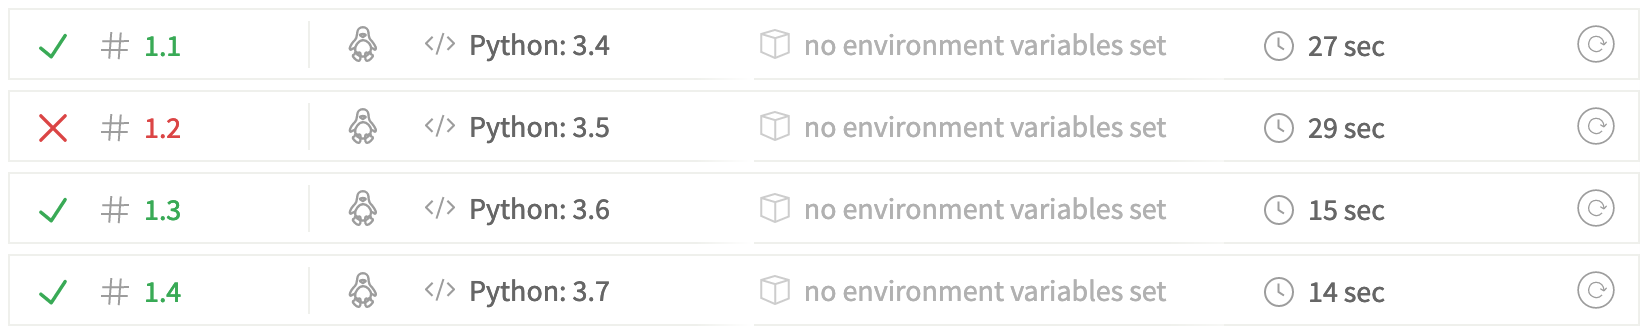
\includegraphics[width=\textwidth]{img/travis1.png}

    \medskip
    Python 3.4: \ttcode{++test_get_stars (testapp.FooTest) ... ok++}

    \medskip
    Python 3.5: \ttcode{!!AttributeError: assert_called!!}

    \medskip
    Python 3.6: \ttcode{++test_get_stars (testapp.FooTest) ... ok++}

    \medskip
    Python 3.7: \ttcode{++test_get_stars (testapp.FooTest) ... ok++}
\end{frame}


% Pitfall #4: Perplexing Build Errors: Missing Method
\begin{frame}[t,fragile]
    \frametitle{Pitfall \#4: Perplexing Build Errors: Missing Method}

    \hspace{-2mm}
    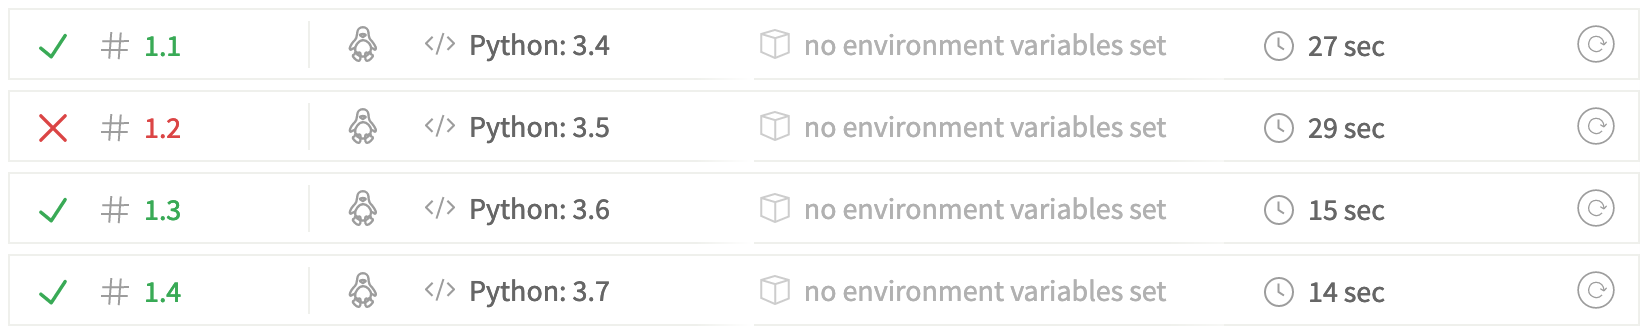
\includegraphics[width=\textwidth]{img/travis1.png}

    \footnotesize
    The \pycode{assert_called()} method is new in Python 3.6.

    \hr{3.5mm}{0mm}

    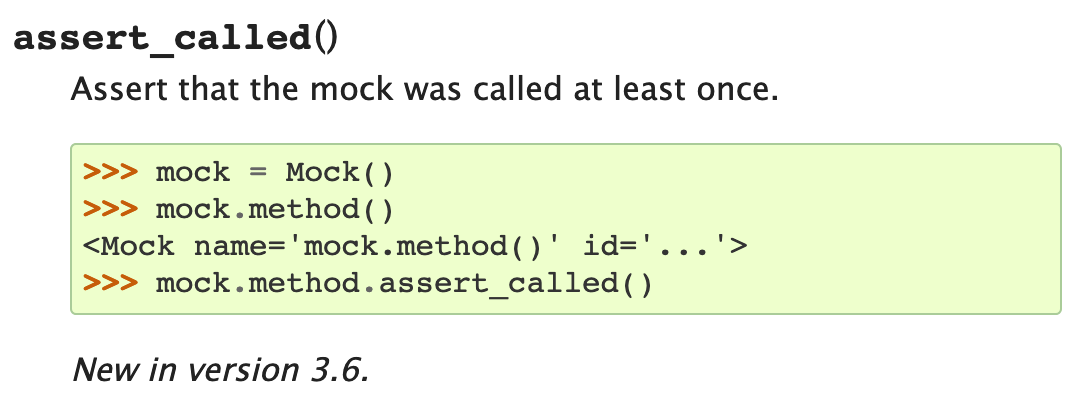
\includegraphics[width=0.65\textwidth]{img/assert-called-doc.png}

    \vspace{-3mm}
    {
    \scriptsize
    See
    \url{https://docs.python.org/3.7/library/unittest.mock.html#unittest.mock.Mock.assert_called}
    }
\end{frame}


% Pitfall #4: Perplexing Build Errors: CPython Commit
\begin{frame}[t,fragile]
    \frametitle{Pitfall \#4: Perplexing Build Errors: CPython Commit}

    \begin{txtenv}[gobble=4]
    cpython/Lib/unittest/mock.py > class NonCallableMock(Base):
    \end{txtenv}

    \vspace{-6mm}

    \hspace{-1mm}
    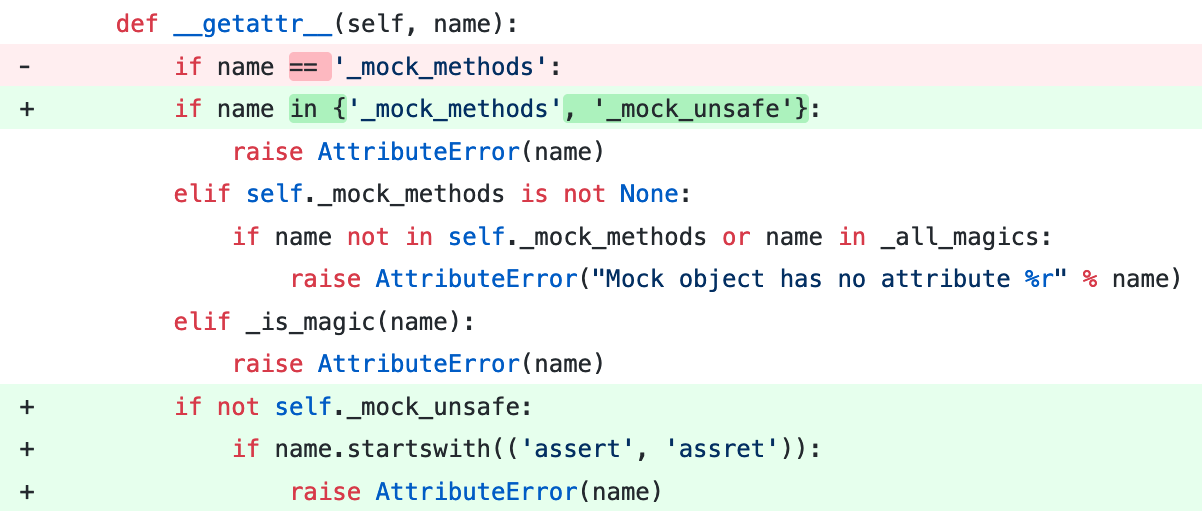
\includegraphics[width=\textwidth]{img/mock-unsafe-diff.png}

    \vspace{-3mm}
    {
        \scriptsize
        See \url{https://github.com/python/cpython/commit/8c14534}
    }

    \hr{2mm}{-0.5mm}

    \footnotesize
    This change in Python 3.5 prevents tests from silently passing when
    we think we have called an assertion method but it does not exist.
\end{frame}


% Pitfall #4: Perplexing Build Errors: Mock Documentation
\begin{frame}[t,fragile]
    \frametitle{Pitfall \#4: Perplexing Build Errors: \ttcode{Mock}
    Documentation}

    The \pycode{assert_called_once()} method is also new in Python 3.6.

    It could also lead to perplexing build errors.

    \hr{3mm}{-1mm}

    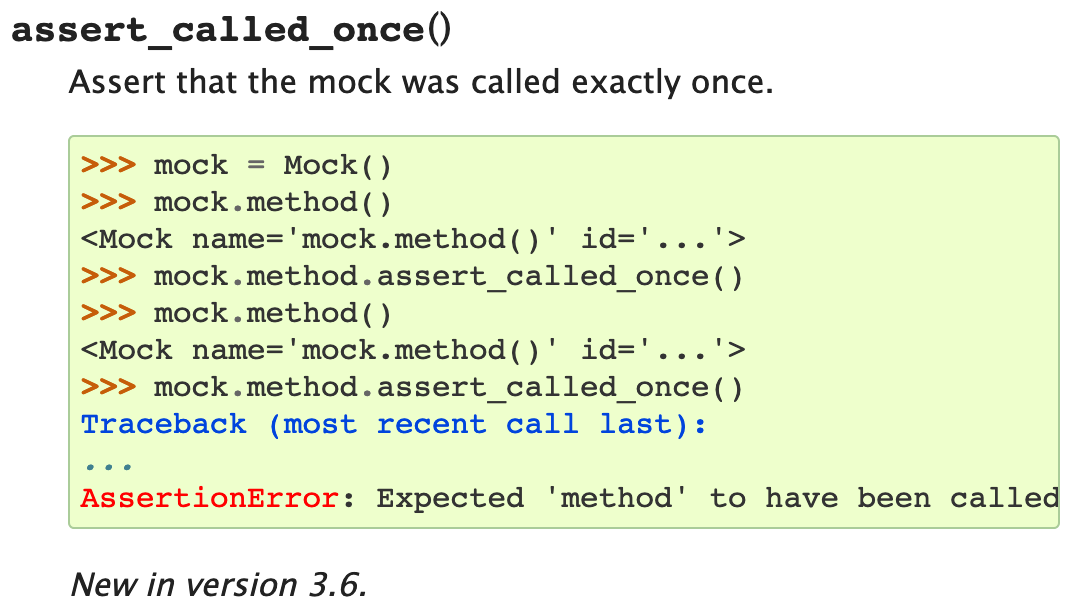
\includegraphics[width=0.75\textwidth]{img/assert-called-once-doc.png}

    \vspace{-2.5mm}
    {
        \tiny
        See
        \url{https://docs.python.org/3.7/library/unittest.mock.html#unittest.mock.Mock.assert_called_once}
    }
\end{frame}


% Pitfal #4: Perplexing Build Errors: Autospeccing
\begin{frame}[t,fragile]
    \frametitle{Pitfall \#4: Perplexing Build Errors: Autospeccing}
    \pyfile[style=footnotesize]{examples/ex3/testapp2.py}
    \hr{1mm}{1mm}
    \footnotesize
    The \pycode{assert_called()} method no longer works silently in
    Python versions 3.4 and 3.5 due to autospeccing.
\end{frame}


% Pitfall #4: Perplexing Build Errors: Autospeccing
\begin{frame}[t,fragile]
    \frametitle{Pitfall \#4: Perplexing Build Errors: Autospeccing}

    \hspace{-2mm}
    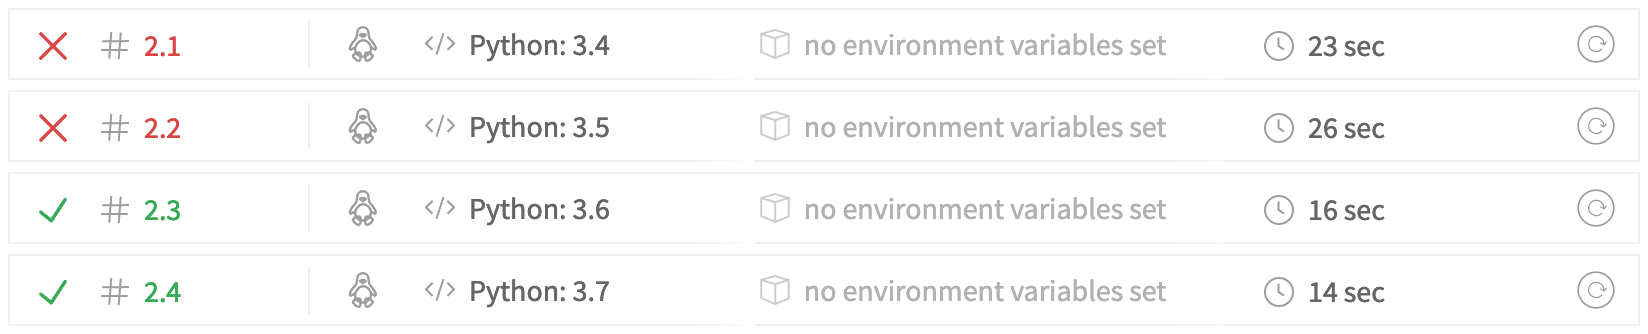
\includegraphics[width=\textwidth]{img/travis2.png}

    \scriptsize

    \medskip
    Python 3.4: \ttcode{!!AttributeError: 'function' object has no
    attribute 'assert_called'!!}

    \medskip
    Python 3.5: \ttcode{!!AttributeError: 'function' object has no
    attribute 'assert_called'!!}

    \medskip
    Python 3.6: \ttcode{++test_get_stars (testapp.FooTest) ... ok++}

    \medskip
    Python 3.7: \ttcode{++test_get_stars (testapp.FooTest) ... ok++}
\end{frame}


% Pitfall #4: Perplexing Build Errors: Solution
\begin{frame}[t,fragile]
    \frametitle{Pitfall \#4: Perplexing Build Errors: Solution}
    \pyfile[style=footnotesize,linerange={1-12,23-26}]{examples/ex3/testapp1.py}
    \hr{0mm}{0mm}
    \footnotesize
    The \pycode{assert_called_once_with()} method is available since
    Python 3.3.
\end{frame}


% Pitfall #5: Asserting Chained Calls: App Code
\begin{frame}[t,fragile]
    \frametitle{Pitfall \#5: Asserting Chained Calls: App Code}
    \pyfile[style=footnotesize]{examples/ex4/app.py}
\end{frame}


% Pitfall #5: Asserting Chained Calls: Unwieldy Test Code
\begin{frame}[t,fragile]
    \frametitle{Pitfall \#5: Asserting Chained Calls: Unwieldy Test Code}
    \pyfile[style=footnotesize,linerange={1-19}]{examples/ex4/testapp.py}
\end{frame}


% Pitfall #5: Asserting Chained Calls: Unwieldy Test Code
\begin{frame}[t,fragile]
    \frametitle{Pitfall \#5: Asserting Chained Calls: Unwieldy Test Code}
    \begin{textblock*}{\textwidth}(4mm,15mm)
        \begin{onlyenv}<1->
        \pyfile[style=scriptsize,linerange={1-1,7-11}]{
            examples/ex4/app.py
        }
        \hr{0mm}{0mm}
        \end{onlyenv}
    \end{textblock*}

    \begin{textblock*}{\textwidth}(4mm,39mm)
        \begin{onlyenv}<1->
        \pyfile[style=scriptsize,linerange={1-1,8-19}]{
            examples/ex4/testapp.py
        }
        \end{onlyenv}
        \begin{onlyenv}<2>
        \hr{0mm}{0mm}
        \end{onlyenv}
    \end{textblock*}

    \begin{textblock*}{\textwidth}(4mm,88.5mm)
        \footnotesize
        \begin{onlyenv}<2>
        We don't need to create the complete list of call objects.
        \end{onlyenv}
    \end{textblock*}
\end{frame}


% Pitfall #5: Asserting Chained Calls: Good Test Code
\begin{frame}[t,fragile]
    \frametitle{Pitfall \#5: Asserting Chained Calls: Good Test Code}
    \begin{textblock*}{\textwidth}(4mm,15mm)
        \begin{onlyenv}<1->
        \pyfile[style=scriptsize,linerange={1-1,7-11}]{
            examples/ex4/app.py
        }
        \hr{0mm}{0mm}
        \end{onlyenv}
    \end{textblock*}

    \begin{textblock*}{\textwidth}(4mm,39mm)
        \begin{onlyenv}<1->
        \pyfile[style=scriptsize,linerange={1-1,8-12,23}]{
            examples/ex4/testapp.py
        }
        \end{onlyenv}
        \begin{onlyenv}<2>
        \hr{0mm}{0mm}
        \end{onlyenv}
    \end{textblock*}

    \begin{textblock*}{\textwidth}(4mm,87mm)
        \footnotesize
        \begin{onlyenv}<2>
        A call object's \pycode{call_list()} method can create the
        complete list of call objects for us.
        \end{onlyenv}
    \end{textblock*}
\end{frame}


% Summary
\begin{frame}[t]
    \frametitle{Summary}
    \small

    \textbf{\#1}

    Patch where an object is looked up, which is not necessarily
    the same place as where it is defined.
    \pause

    \bigskip

    \textbf{\#2}

    Do not create a new mock to assign to a mock's
    \pycode{return_value}. A mock's \pycode{return_value} is already
    a mock by default. Just use it and configure it.
    \pause

    \bigskip

    \textbf{\#3}

    Do not set a \pycode{tuple}, \pycode{list}, or \pycode{dict} as
    the \pycode{return_value} of a \pycode{MagicMock} object only to
    make it subscriptable. A \pycode{MagicMock} object is already
    subscriptable.
\end{frame}

\begin{frame}[t]
    \frametitle{Summary}
    \small
    \textbf{\#4}

    Do not use \pycode{assert_called()} or \pycode{assert_called_once()}
    if you are still supporting Python 3.4. Use
    \pycode{assert_called_once_with()} instead.
    \pause

    \bigskip

    \textbf{\#5}

    Do not create a long list of \pycode{mock.call} objects to mimic
    \pycode{mock_calls} of a mock's chained calls. Use
    \pycode{call_list()} to generate the list for you.
\end{frame}


% Thank You.
\begin{frame}
    \begin{center}
        \Huge
        Thank You
    \end{center}
\end{frame}

\end{document}
